\documentclass{beamer}

\mode<presentation> {

%\usetheme{default}
%\usetheme{AnnArbor}
%\usetheme{Antibes}
%\usetheme{Bergen}
%\usetheme{Berkeley}
%\usetheme{Berlin}
%\usetheme{Boadilla}
%\usetheme{CambridgeUS}
%\usetheme{Copenhagen}
%\usetheme{Darmstadt}
%\usetheme{Dresden}
%\usetheme{Frankfurt}
%\usetheme{Goettingen}
%\usetheme{Hannover}
%\usetheme{Ilmenau}
%\usetheme{JuanLesPins}
%\usetheme{Luebeck}
\usetheme{Madrid}
%\usetheme{Malmoe}
%\usetheme{Marburg}
%\usetheme{Montpellier}
%\usetheme{PaloAlto}
%\usetheme{Pittsburgh}
%\usetheme{Rochester}
%\usetheme{Singapore}
%\usetheme{Szeged}
%\usetheme{Warsaw}


%\usecolortheme{albatross}
%\usecolortheme{beaver}
%\usecolortheme{beetle}
%\usecolortheme{crane}
%\usecolortheme{dolphin}
%\usecolortheme{dove}
%\usecolortheme{fly}
%\usecolortheme{lily}
%\usecolortheme{orchid}
%\usecolortheme{rose}
%\usecolortheme{seagull}
%\usecolortheme{seahorse}
%\usecolortheme{whale}
%\usecolortheme{wolverine}

%\setbeamertemplate{footline} % To remove the footer line in all slides uncomment this line
%\setbeamertemplate{footline}[page number] % To replace the footer line in all slides with a simple slide count uncomment this line

%\setbeamertemplate{navigation symbols}{} % To remove the navigation symbols from the bottom of all slides uncomment this line
}

\usepackage{graphicx} % Allows including images
\usepackage{booktabs} % Allows the use of \toprule, \midrule and \bottomrule in tables
\usepackage{amsfonts}
\usepackage{mathrsfs}
\usepackage{amsmath,amssymb,graphicx}
\usepackage{hyperref} 
\usepackage{bm}
 
%----------------------------------------------------------------------------------------
%	TITLE PAGE
%----------------------------------------------------------------------------------------

\title["2.4"]{2.4: Properties of the Sample Mean and the Sample Autocorrelation Function}

\author{Taylor} 
\institute[UVA] 
{
University of Virginia \\
\medskip
\textit{} 
}
\date{} 

\begin{document}
%----------------------------------------------------------------------------------------

\begin{frame}
\titlepage 
\end{frame}
%----------------------------------------------------------------------------------------

\begin{frame}
\frametitle{Motivation}

$X_t$ is characterized by $\mu$ and $\gamma(\cdot)$. This chapter talks about model-free estimators of these quantities. Both the formulas for the estimators, and their sampling distributions. 
\end{frame}

%----------------------------------------------------------------------------------------

\begin{frame}
\frametitle{Estimating the Mean}

We estimate the mean with $\bar{X} = n^{-1}\sum_iX_i$. It is unbiased
\[
E[\bar{X}] = n^{-1}(E[X_1] + \cdots + E[X_n]) = \mu
\]
by linearity of $E[\cdot]$ and stationarity, and it's mean squared error (MSE) is
\begin{align*}
\text{MSE}(\bar{X}) &= \text{Var}(\bar{X}) && \text{defn}\\
&= \text{Cov}\left(\sum_{i=1}^n n^{-1}X_i , \sum_{j=1}^n n^{-1}X_j \right) && \text{defn} \\
&= n^{-2} \sum_{i=1}^n\sum_{j=1}^n \text{Cov}(X_i,X_j) && \text{bilinearity of cov} \\
&= n^{-2} \sum_{h=-(n-1)}^{n-1} (n - |h|) \gamma_X(h) && \text{count diagonally : $h = i-j$} \\
&= n^{-1} \sum_{h} \left(1 - \frac{|h|}{n} \right) \gamma_X(h)
\end{align*}


\end{frame}

%----------------------------------------------------------------------------------------


\begin{frame}
\frametitle{Note}
\begin{block}{1.)} 
\[
\text{Var}(\bar{X}) = n^{-1} \sum_{h=-(n-1)}^{(n-1)} \left(1 - \frac{|h|}{n} \right) \gamma_X(h) \to 0 
\]
as $n \to \infty$ if $\gamma(h) \to 0$, and \\
\end{block}

\begin{block}{2.)}
\[
n\text{Var}(\bar{X}) \to \sum_{h=-\infty}^{\infty} \gamma(h)
\]
as $n \to \infty$ if $\sum_{h=-\infty}^{\infty} |\gamma_X(h)| < \infty$ 

\href{https://goo.gl/wVjL7b}{\beamergotobutton{ Proof}}
\end{block}
\end{frame}

%----------------------------------------------------------------------------------------


\begin{frame}
\frametitle{Inference for $\mu$}

We are usually interested if $\mu > 0$ or not. This affects our decision on whether or not to buy an asset. To construct confidence intervals and perform hypothesis tests, we need the sampling distribution of $\bar{X}$.
\newline

If our time series is weakly stationary then 
\[
\bar{X} \overset{\text{approx.}}{\sim} \text{Normal}\left(\mu, n^{-1} \sum_{h=-n}^n  \gamma_X(h)\right).
\]
for large $n$. Or, if we assume all our noise terms are Normally distributed, then 
\[
\bar{X} \sim \text{Normal}\left(\mu, n^{-1} \sum_{h=-n}^n \left(1 - \frac{|h|}{n} \right) \gamma_X(h)\right)
\]
exactly. However, we usually don't know the true autocovariance function.
\end{frame}

%----------------------------------------------------------------------------------------


\begin{frame}
\frametitle{Inference for $\mu$}

We can estimate $V^2 = \sum_{h=-n}^n \left(1 - \frac{|h|}{n} \right) \gamma_X(h)$ with 
\[
\hat{V}^2 = \sum_{h=-n}^n \left(1 - \frac{|h|}{n} \right) \hat{\gamma}_X(h).
\]
A $(1-\alpha)$\% confidence interval is $\bar{x} \pm z_{\alpha/2}\sqrt{v^2/n}$, and a hypothesis test against the null of $H_0: \mu = 0$ can use the test statistic $\sqrt{n}\bar{x}/\hat{v}$ (rejection region depends on the alternative hypothesis).


\end{frame}

%----------------------------------------------------------------------------------------


\begin{frame}
\frametitle{Example}
$\bar{X} = 0.006153473$!

\begin{center}
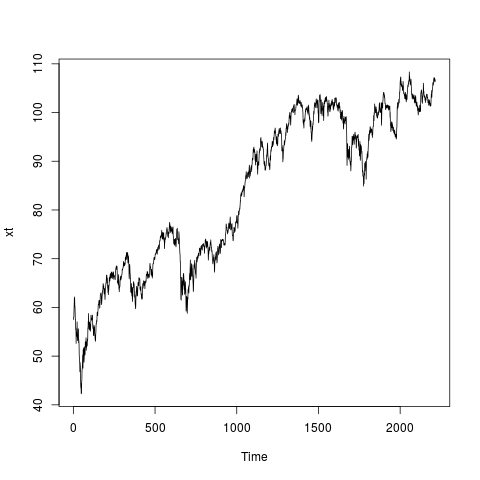
\includegraphics[width=44mm]{/home/taylor/UVa/all_teaching/4170_slides/2/2.4/pics/Rplot.png}
\end{center}

\end{frame}

%----------------------------------------------------------------------------------------


\begin{frame}[fragile]
\frametitle{Example}

So we're interested in $\mu$. The previous theorems are useful because they tell us our estimates get very close to the true mean, but also that future average returns will be arbitrarily close to the true mean. Buying and holding is profitable if $\mu > 0$.
\newline

95\% Confidence interval: 
\begin{verbatim}
> xbar - zAlphaOverTwo * sqrt(asympVar) #lower
[1] -0.0273102
> xbar + zAlphaOverTwo * sqrt(asympVar) #upper
[1] 0.03961714
\end{verbatim}

Try different approximations for the standard deviation, try raising $\alpha$, or try lower confidence intervals.
\end{frame}

%----------------------------------------------------------------------------------------


\begin{frame}
\frametitle{Estimating $\gamma$ and $\rho$}

If we have a time series, knowing about the mean is great. However, we can increase the accuracy of our predictions if we also learn about the time structure via $\gamma(\cdot)$ or $\rho(\cdot)$.
\newline

Recall that 
\[
\hat{\gamma}(h) = n^{-1}\sum_{t=1}^{n-|h|}(X_{t+|h|}-\bar{X}_n)(X_t - \bar{X}_n)
\]
and 
\[
\hat{\rho}(h) = \frac{\hat{\gamma}(h) }{\hat{\gamma}(0)}.
\]

\end{frame}

%----------------------------------------------------------------------------------------

\begin{frame}
\frametitle{NND of Autocovariance}

Proving a matrix is non-negative definite often involves finding a square root matrix. When you can do that, writing the quadratic form becomes a square norm that can't be negative. 
\newline

Often times the autocovariance matrix is positive definite ($>0$), too (page 52).
\newline

Lastly, notice for $h$ large or $n$ small, higher order autocovariance estimates are unreliable. ``Jenkins (1976), p. 33 who suggest that $n$ should be at least about $50$ and $h \le n/4$."
\newline

Also, we always divide by $n$. If we divided sums of squares by $(n-h)$, this proof wouldn't work.

\end{frame}

%----------------------------------------------------------------------------------------

\begin{frame}
\frametitle{NND of Autocovariance}

Notice that 
\[
\hat{\Gamma}_k = n^{-1} TT'
\]
where
\[
\hat{\Gamma}_k
=
\left[\begin{array}{cccc}
\hat{\gamma}(0) & \hat{\gamma}(1) & \cdots & \hat{\gamma}(k-1)\\
\hat{\gamma}(1) & \hat{\gamma}_(0) & \cdots & \hat{\gamma}(k-2)\\
\vdots & \vdots & \cdots & \vdots \\
\hat{\gamma}(k-1) & \hat{\gamma}(k-1) & \cdots & \hat{\gamma}(0)
\end{array}\right]
\]
and $T$ is equal to 
\[
\left[\begin{array}{cccccccc}
0 & \cdots  & 0 & 0 & X_1 - \bar{X} & X_2-\bar{X} & \cdots & X_k - \bar{X}\\
0 & \cdots  & 0 & X_1-\bar{X} & X_2-\bar{X} & \cdots & X_k-\bar{X} & 0\\
\vdots &  &  &  &  &  &  & \vdots \\
0 & X_1 - \bar{X}  &  X_2 - \bar{X} & \cdots & X_k - \bar{X} & 0 & \cdots & 0\\
\end{array}\right]
\]
So for any weight vector $w$, $w'\hat{\Gamma}_k w = n^{-1}(T'w)'(T'w) = n^{-1} c'c \ge 0$.



\end{frame}

%----------------------------------------------------------------------------------------
\begin{frame}
\frametitle{Bartlett's Formula}

The sampling distribution of $\hat{\rho}$ is very difficult to find exactly. Approximately, when $n$ is large, though, we have $\hat{\bm{\rho} }_k = (\hat{\rho}(1), \ldots, \hat{\rho}_k)'$
\[
\hat{\bm{\rho} }_k \overset{\text{approx.}}{\sim} \text{N}(\bm{\rho}, n^{-1}\bm{W} )
\]

The coefficients of $\bm{W}$ are given by {\bf Barlett's formula} (not reproduced here). Two versions of this formula are given on page 53. 
\newline

We used this formula once before: chapter 1.6 tested residuals for independence (example 2.4.2 mentions this). Under the null that $\bm{\rho} = \bm{0}$, the asymptotic covariance matrix simplifies to $n^{-1}I_n$. 

\end{frame}



\end{document} 